\documentclass[]{beamer}
\mode<presentation>{
  %% \usetheme[compress]{Berlin}
}
%% packages
\usepackage{zhspacing}
\zhspacing
\usepackage{graphics}
\usepackage{listings}
\lstset{
  basicstyle=\ttfamily\tiny,
  numbers=left
}
\usepackage{tabularx}
\usepackage{booktabs}
\usepackage{enumerate}

%% meta info
\title{Finding Dominators in Flowgraphs}
\subtitle{The Lengauer-Tarjan Algorithm}
\author[SuXing~pysuxing@gmail.com]{SuXing}
\institute{TOW}
\date{\today}

%% slides
\begin{document}
\setlength{\parindent}{0pt}

\frame{\titlepage}
\frame{\tableofcontents}

\section{Preliminaries}
\frame{\tableofcontents[currentsection]}

\begin{frame}
  \frametitle{Flowgraph}
  \begin{definition}
    \alert{Flowgraph} is a graph $G=(V, E)$ that satisfies that $\exists r \in V$,
    for $\forall n \in V$ there is a path from $r$ to $n$
  \end{definition}
  \vspace{1em}\pause
  We call $r \in V$ the \alert{entry} of $G=(V, E)$, written as $G=(V, E, r)$

  \vspace{1em}\pause
  e.x. CFG is a flowgraph            % figure here
\end{frame}

\begin{frame}
  \frametitle{Dominance}
  \begin{definition}
    For two vertices $a, b \in V$, we say $a$ \alert{dominates} $b$ if all paths from $r$ to $b$
    go through $a$, written as $a \succeq b$. If $a$ dominates $b$ and $a \neq b$, we say $a$
    \alert{strictly dominates} $b$, written as $a \succ b$
  \end{definition}

  \pause
  Dominance is a binary relationship defined on $V$ and it's
  \begin{itemize}
    \item (ir)reflexive: $a \succeq a$, $a \nsucc a$
    \item asymmetric: $a \succeq b \Rightarrow b \nsucceq a$
    \item transitive: $a \succeq b$ and $b \succeq c$ $\Rightarrow$ $a \succeq c$
  \end{itemize}
\end{frame}

\begin{frame}
  \frametitle{Dominators \& Immediate Dominator}
  \begin{definition}
    A vertex $a$'s \alert{dominators} is a vertex set made up of all vertices that dominate $a$,
    written as $$Dom(a)=\{ b | b \in V, b \succeq a \}$$
  \end{definition}
  \pause
  \begin{definition}
    If $b \in Dom(a)$ satisfies $\forall c \in Dom(a)$, $c \succeq b$, we say $b$
    \alert{immediate dominates} $a$, written as $b=idom(a)$
  \end{definition}
\end{frame}

\section{Why Dominators}
\frame{\tableofcontents[currentsection]}

\begin{frame}
  \frametitle{Why Dominators?}
  \centerline{\Large Least but not last, we need it to construct SSA from CFG!}

  \vspace{2em}\pause
  But we won't cover this topic here
\end{frame}

\section{The Lengauer-Tarjan Algorithm}
\frame{\tableofcontents[currentsection]}

\begin{frame}
  \frametitle{Dominance Tree}
  \begin{definition}
    A graph $G=(V, E, r)$'s \alert{Dominance Tree } $DT=(V_D, E_D, r_D)$ is constructed as follows:
    $$V_D=V, E_D=\{ (idom(a), a) | a \in V, a \neq r \}, r_D=r$$
  \end{definition}

  \pause
  Insight: All $a$'s dominators form a dominance chain, and the nearest vertex to $a$ itself is $idom(a)$.
  Any $a$'s ancestor in $DT$ is its dominator in $G$
\end{frame}

\begin{frame}
  \frametitle{The Problem}
  What's the problem now?

  \vspace{1em}\pause
  \centerline{calc $Dom(a)$ for each $a \in V$}
  \centerline{$\Downarrow$}
  \pause
  \centerline{calc $DT$ from $G$}
  \centerline{$\Downarrow$}
  \pause
  \centerline{calc $idom(a)$ for each $a \in V$}

  \vspace{1em}\pause
  Here comes the \alert{Lengauer-Tarjan} algorithm!
\end{frame}

\begin{frame}
  \frametitle{The Lengauer-Tarjan Algorithm}
  The Lengauer-Tarjan(LT) algorithm is the classical one in dominance algorithms,
  published in TOPLAS 1997\cite{Lengauer1979} and works in $O(E \log N)$ time

  \vspace{1em}\pause
  Some improvements has been made since then
  \cite{Harel1985},\cite{Buchsbaum1998a},\cite{Buchsbaum1998},\cite{Alstrup1999},
  \cite{Cooper2001},\cite{Georgiadis2004},
  see the references page
\end{frame}

\begin{frame}
  \frametitle{DFS Spanning Tree}
  Graph $G=(V, E, r)$ has a \alert{DFS Spanning Tree(DFST)}
  rooted at $r$, and each vertex is assigned a number indicating its
  traversal order(traversed in preorder DFS).

  \pause
  \begin{columns}
    \begin{column}{.65\textwidth}
      \begin{figure}
        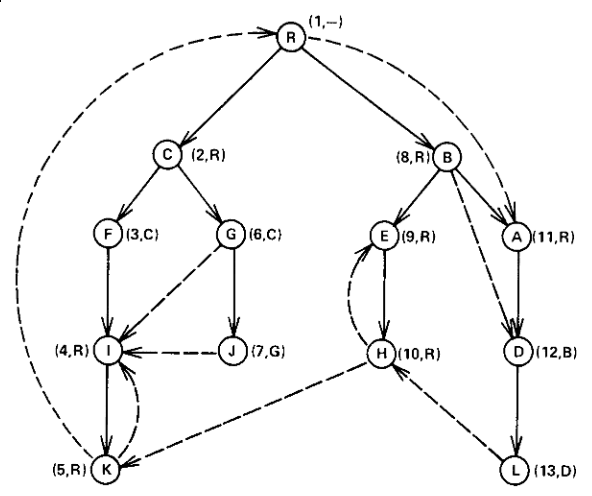
\includegraphics[height=.55\textheight]{figures/dfst}
      \end{figure}
    \end{column}
    \begin{column}{.35\textwidth}
      \begin{itemize}
        \item tree edges%: all edges in DFST
        \item advancing edges%: edges to proper descendants
        \item retreating edges%: edges to proper ancestors and to self
        \item crossing edges (always \alert{right to left})%: edges between vertices, neither of which is not
          %an ancestor of the other 
      \end{itemize}
    \end{column}
  \end{columns}
\end{frame}

\begin{frame}
  \frametitle{Semidominator}
  To calc $idom(w)$, we calc $w$'s \alert{semidominator} $sdom(w)$ first

  \pause
  \begin{definition}
    For a vertex $w \neq r \in V$, its \alert{semidominator} is defined as below:

    $sdom(w) = \min \{ v | $ there is a path $v=v_0, v_1, \cdots, v_k=w$ such that
    $v_i>w$ for $1 \leq i \leq k-1 \}$
  \end{definition}

  \pause
  $sdom(w)$ can hopefully be $idom(w)$, but \alert{not} necessarily. That's what 'semi' means.
\end{frame}

\begin{frame}
  \frametitle{Semidominator (cont.)}
  \begin{figure}
    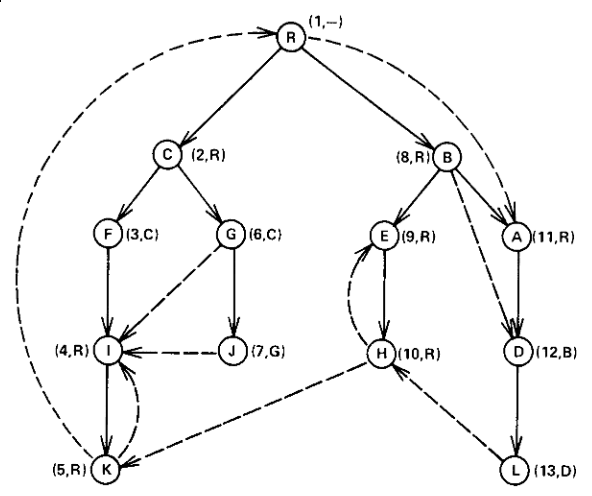
\includegraphics[height=.55\textheight]{figures/dfst}
  \end{figure}
\end{frame}

\begin{frame}
  \frametitle{$w$, $idom(w)$ and $sdom(w)$}
  Some facts without formal proof
  \begin{itemize}
    \item For any vertex $w \neq r$, $sdom(w)$ is a proper ancestor of $w$
    \item For any vertex $w \neq r$, $idom(w)$ is a proper ancestor of $w$
    \item For any vertex $w \neq r$, $idom(w)$ is a ancestor of $sdom(w)$
  \end{itemize}
\end{frame}

\begin{frame}
  \frametitle{Theorem of Semidominator}
  \begin{theorem}
    For any vertex $w \neq r$,

    $sdom(w) = \min ( \{ v | (v,w) \in E$ and $v<w \} \cup \{ sdom(u) | u>w$ and
    there is an dege $(u,w)$ such that v is reachable from $v\})$
  \end{theorem}

  \vspace{1em}\pause
  Feel dizzy? Uh ...\hfill
\includegraphics[height=.3\textheight]{figures/dizzy.jpeg}
\end{frame}

\begin{frame}
  \frametitle{Theorem of Semidominator (cont.)}
  \begin{figure}
    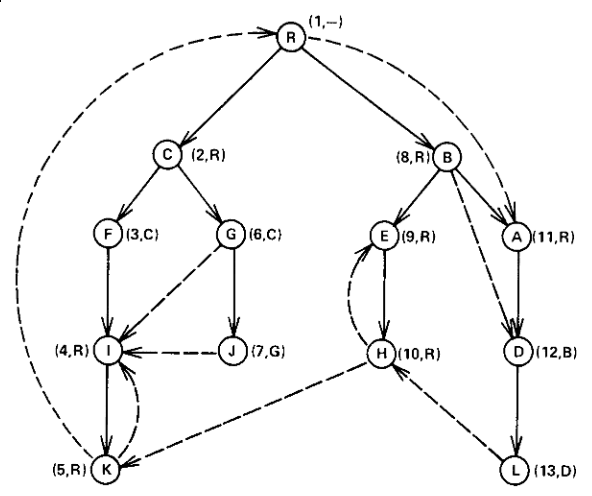
\includegraphics[height=.55\textheight]{figures/dfst}
  \end{figure}
\end{frame}

\begin{frame}
  \frametitle{Theorem of Dominators}
  \begin{theorem}
    Let $w \neq r$ and let $u$ be a vertex for which $sdom(u)$ is minimum
     among vertices $u$ satisfying $sdom(w)$ is proper ancestor of $u$ and
     $u$ is ancestor of $w$, then
     \begin{equation*}
       idom(w)=\left\{
       \begin{array}{ll}
         {sdom(w)} &\text{if $sdom(w)=sdom(u)$}\\
         {idom(u)} &\text{otherwise}
       \end{array}  
       \right.
     \end{equation*}
  \end{theorem}
\end{frame}

\section{Summary}
\frame{\tableofcontents[currentsection]}

\begin{frame}
  \frametitle{Summary}
  \begin{itemize}
    \item Some basic definitions in graph theory
    \item The dominance problem and its value
    \item The Lengauer-Tarjan Algorithm, all proof detail omitted
  \end{itemize}
\end{frame}

\begin{frame}
  \frametitle{References}
  \bibliographystyle{plain}
  {\tiny \bibliography{slides.bib}}
\end{frame}

\frame{\centerline{\Huge Q\&A}}

\end{document}
